Many hardware evolution happened between the development of Wolfenstein 3D (Mid-1991) and the start of the development of Doom. The consumer machine had new CPUs, new Bus, new Sound Cards. The machine were almost twice as powerful as the year before. The development environment had also changed with powerful workstation, compilers and DOS extenders. id Software made the audacious decision to start from a clean sheet.\\

\section{Intel 486}
By may 1992, the Intel 386 was being replaced by a new version, the 486. The increase in operatin frequency was substancial for the high end model running at 50Mhz but most 486 ran at the same speed at the 386: 25Mhz and 33Mhz. The revolutionary design of the CPU 
\begin{figure}[H]
\centering
  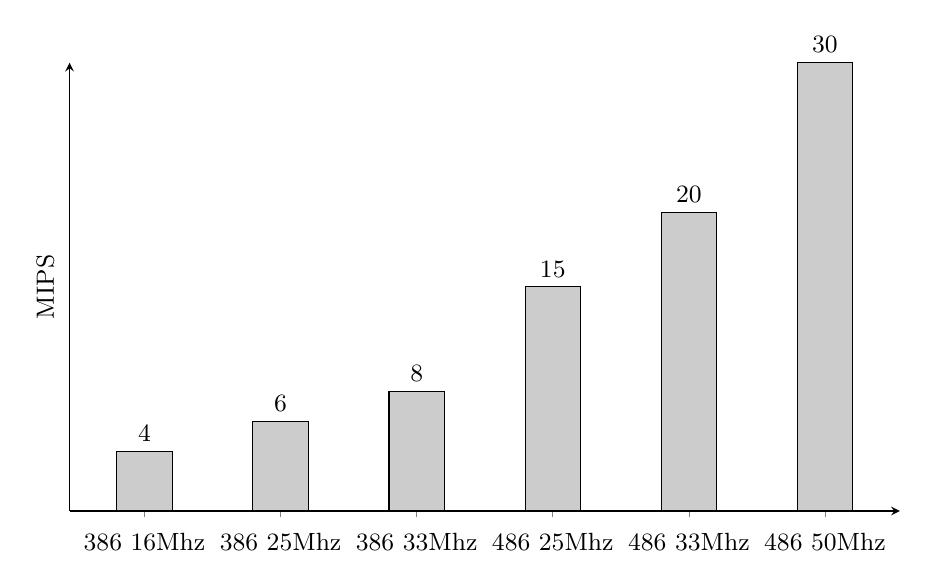
\begin{tikzpicture}[font=\small]
    \begin{axis}[
      width=1.0\textwidth,
      height=0.6\textwidth,
      ybar,
      bar width=20pt,
      ylabel={MIPS},
      ymin=0,
      ytick=\empty,
      xtick=data,
      axis x line=bottom,
      axis y line=left,
      enlarge x limits=0.11,
      symbolic x coords={386 16Mhz,386 25Mhz,386 33Mhz,486 25Mhz,486 33Mhz,486 50Mhz},
      xticklabel style={anchor=base,yshift=-\baselineskip},
      nodes near coords={\pgfmathprintnumber\pgfplotspointmeta}
    ]
      \addplot[fill=black!20,draw=black] coordinates {
        (386 16Mhz,4)
        (386 25Mhz,6)
        (386 33Mhz,8)
        (486 25Mhz,15)
        (486 33Mhz,20)
        (486 50Mhz,30)
      };
    \end{axis}
   
   \end{tikzpicture}
   \caption{Comparison\protect\footnotemark of CPUs with MIPS \protect\footnotemark.}
 \end{figure}
\footnotetext{Source: "Roy Longbottom's PC Benchmark Collection: http://www.roylongbottom.org.uk/mips.htm".}
















\subsection{Pipeline}
\subsection{Cache}
four-way set-associative\\
\subsection{Precaching (cachelines)}














\section{Overdrive, 486 DX2 66Mhz}
\begin{figure}[H]
\centering
  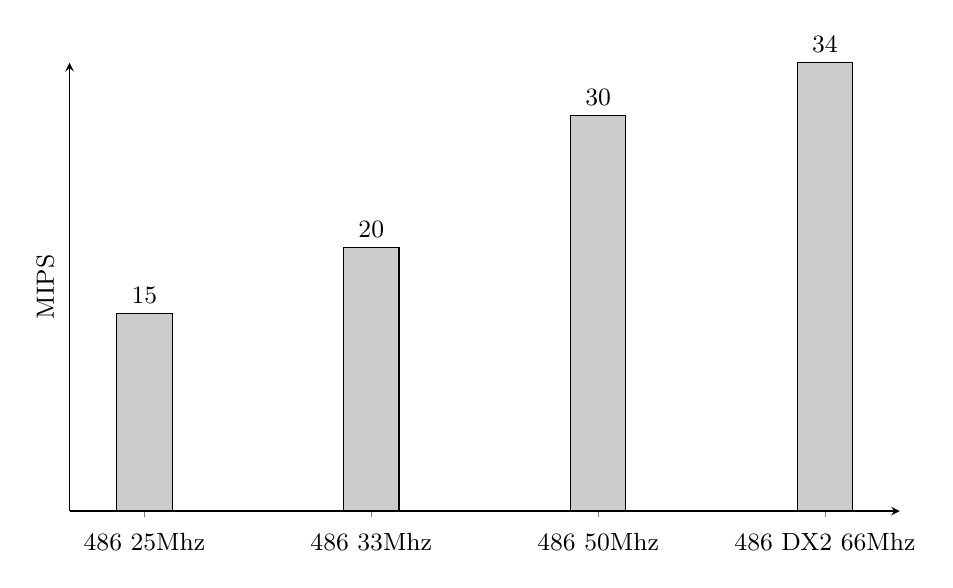
\begin{tikzpicture}[font=\small]
    \begin{axis}[
      width=1.0\textwidth,
      height=0.6\textwidth,
      ybar,
      bar width=20pt,
      ylabel={MIPS},
      ymin=0,
      ytick=\empty,
      xtick=data,
      axis x line=bottom,
      axis y line=left,
      enlarge x limits=0.11,
      symbolic x coords={486 25Mhz,486 33Mhz,486 50Mhz,486 DX2 66Mhz},
      xticklabel style={anchor=base,yshift=-\baselineskip},
      nodes near coords={\pgfmathprintnumber\pgfplotspointmeta}
    ]
      \addplot[fill=black!20,draw=black] coordinates {
        (486 25Mhz,15)
        (486 33Mhz,20)
        (486 50Mhz,30)
        (486 DX2 66Mhz,34)
      };
    \end{axis}
   
   \end{tikzpicture}
   \caption{Comparison\protect\footnotemark of CPUs with MIPS \protect\footnotemark.}
 \end{figure}
\footnotetext{Source: "Roy Longbottom's PC Benchmark Collection: http://www.roylongbottom.org.uk/mips.htm".}

\section{Dos Extender}
\section{NeXT}
After leaving Apple in 1985, Steve Jobs founded a new company called NeXT, Inc. which unveiled its first product, the NeXT Computer, at a gala event in 1988. The NeXT combined powerful hardware and software in ways that had never been done before.  First, NeXT based its machine on the Motorola 68030 processor running at a screaming 25 Mhz and coupled it with the first built-in Digital Signal Processor.  NeXT's system software was designed to rival the best offerings of the Macintosh and PC: NeXT used the rock-solid UNIX operating system and added its own elegant, proprietary graphical user interface.  NeXT was also the first computer company to ship a built-in 256 MB magneto-optical storage medium.  Boasting a high-resolution display, built-in Ethernet, CD-quality sound, and multimedia e-mail, the NeXT Computer was packaged in a stunning one-foot by one-foot black magnesium cube.\\
\par
In 1990, NeXT unveiled faster workstations running at 25MHz on the Motorola 68040. Affectionately called "the slab," the NeXTstation had a black and white display while the NeXTstation Color displayed 4,096 colors from a palette of 16 million colors. A new version of the Cube offered a 32-bit true-color display.
Spring of 1992 brought about the end of NeXT's optical disk, but NeXT also introduced upgraded workstations, the NeXTstation Turbo and Turbo Color running at 33MHz. NeXT also began offering a color printer and a standard CD-ROM drive. Foreshadowing its exit from the hardware business, the company announced it had begun working on NeXTstep for Intel.\\
\par
NeXT stopped manufacturing hardware in 1993 to become a software-only vendor, selling NeXTSTEP as a combination operating system and object-oriented development environment. NeXTstep for Intel became a popular product among large companies and especially financial institutions for rapidly developing and deploying custom software. \\
\par
Apple Computer bought NeXT in 1996 after its own efforts to upgrade the Macintosh operating system failed.  After the sale, Steve Jobs first began working as an advisor but was later appointed acting-CEO, and then finally CEO of the company.  NeXTSTEP lives on as the heart of Mac OS X.\\
\par




\section{Gravis UltraSounds}
\section{Sound Blaster 16}